%% Dokumenteinstellungen %%%%%%%%%%%%%%%%%%%%%%%%%%%%%%%%%%%%
\documentclass[a4paper,oneside,12pt,ngerman]{scrartcl}

%% Deutsche Anpassungen %%%%%%%%%%%%%%%%%%%%%%%%%%%%%%%%%%%%%
\usepackage[ngerman]{babel}
\usepackage[T1]{fontenc}
\usepackage[ansinew]{inputenc}
\usepackage{lmodern} %Type1-Schriftart f�r nicht-englische Texte
\usepackage{booktabs}	% sch�nere tabellen

%% Packages f�r Grafiken & Abbildungen %%%%%%%%%%%%%%%%%%%%%%
\usepackage{graphicx} %%Zum Laden von Grafiken
%\usepackage{subfig} %%Teilabbildungen in einer Abbildung
%\usepackage{tikz} %%Vektorgrafiken aus LaTeX heraus erstellen


%% Packages f�r Formeln %%%%%%%%%%%%%%%%%%%%%%%%%%%%%%%%%%%%%
\usepackage{amsmath}
\usepackage{amsthm}
\usepackage{amsfonts}


%% Andere Packages %%%%%%%%%%%%%%%%%%%%%%%%%%%%%%%%%%%%%%%%%%
%\usepackage{a4wide} %%Kleinere Seitenr�nder = mehr Text pro Zeile.
\usepackage{fancyhdr} %%Fancy Kopf- und Fu�zeilen
%\usepackage{longtable} %%F�r Tabellen, die eine Seite �berschreiten
\usepackage{lastpage}
\usepackage[raggedright]{subfigure}
\usepackage[final]{pdfpages}
\includepdfset{pages=-,noautoscale}

%%%%%%%%%%%%%%%%%%%%%%%%%%%%%%%%%%%%%%%%%%%%%%%%%%%%%%%%%%%%%
%% TODO
%%%%%%%%%%%%%%%%%%%%%%%%%%%%%%%%%%%%%%%%%%%%%%%%%%%%%%%%%%%%%
% 
% 
%%%%%%%%%%%%%%%%%%%%%%%%%%%%%%%%%%%%%%%%%%%%%%%%%%%%%%%%%%%%%



%%%%%%%%%%%%%%%%%%%%%%%%%%%%%%%%%%%%%%%%%%%%%%%%%%%%%%%%%%%%%
%% Optionen / Modifikationen
%%%%%%%%%%%%%%%%%%%%%%%%%%%%%%%%%%%%%%%%%%%%%%%%%%%%%%%%%%%%%
%%%%%%%%%%%%%%%%%%%%%%%%%%%%%%%%%%%%%%%%%%%%%%%%%%%%%%%%%%%%%
%%                                                         %%
%%                     EINSTELLUNGEN                       %%
%%                                                         %%
%%%%%%%%%%%%%%%%%%%%%%%%%%%%%%%%%%%%%%%%%%%%%%%%%%%%%%%%%%%%%

%%%%%%%%%%%%%%%%%%%%%%%%%%%%%%%%%%%%%%%%%%%%%%%%%%%%%%%%%%%%%
%% HYPER REF
%%%%%%%%%%%%%%%%%%%%%%%%%%%%%%%%%%%%%%%%%%%%%%%%%%%%%%%%%%%%%
\usepackage[
hyperindex=true,
colorlinks=true,
linkcolor=black,
citecolor=black,
filecolor=black,
menucolor=black,
urlcolor=cyan,
breaklinks=true,
bookmarks=true,
bookmarksopen=false,
bookmarksnumbered=false,
pdfhighlight=/O,
]{hyperref}

%%%%%%%%%%%%%%%%%%%%%%%%%%%%%%%%%%%%%%%%%%%%%%%%%%%%%%%%%%%%%
%% FANCY HEADERS
%%%%%%%%%%%%%%%%%%%%%%%%%%%%%%%%%%%%%%%%%%%%%%%%%%%%%%%%%%%%%
% --- Kopf- und Fusszeilen - {} = rechts (gerade), [] = links (ungerade)
% letzte seite: \pageref{LastPage}
% doppelseitig:
%\lhead{Elektronik: \textbf{Oszilatorschaltungen}}	\chead{}		\rhead{Cyril Stoller und Hannes Stauffer}
%\lfoot{\today}	\cfoot{}		\rfoot{Seite \thepage\ von \pageref{LastPage}}

% einseitig:
%\lhead{\rightmark}			\chead{}					\rhead{}
%\lfoot{\leftmark}			\cfoot{}					\rfoot{Seite \thepage\ von \pageref{\LastPage}}

%\setlength{\headrulewidth}{0.4pt}
%\setlength{\footrulewidth}{0.4pt}


% Formeln r�misch nummerieren
\renewcommand{\theequation}{\Roman{equation}} 

% "Formel" statt "Gleichung"
\def\equationname{Formel}

%%%%%%%%%%%%%%%%%%%%%%%%%%%%%%%%%%%%%%%%%%%%%%%%%%%%%%%%%%%%%
%% DOKUMENT
%%%%%%%%%%%%%%%%%%%%%%%%%%%%%%%%%%%%%%%%%%%%%%%%%%%%%%%%%%%%%
\begin{document}

\title{Projektarbeit: Buckconverter (Step-Down)}
\date{\today}
\author{Cyril Stoller, Jascha Haldemann, Marcel B�rtschi, Nicola K�ser}
\maketitle


%\pagestyle{fancy} %%Ab hier die Kopf-/Fusszeilen: headings / fancy / ...

\vspace{1cm}


%%%%%%%%%%%%%%%%%%%%%%%%%%%%%%%%%%%%%%%%%%%%%%%%%%%%%%%%%%%%%
%%                                                         %%
%%         Kapitel / Hauptteil des Dokumentes              %%
%%                                                         %%
%%%%%%%%%%%%%%%%%%%%%%%%%%%%%%%%%%%%%%%%%%%%%%%%%%%%%%%%%%%%%

\section{Ziel/Anforderungen}
Mithilfe der im Unterricht erarbeiteten Theorie und der Application Note von Infineon sollen alle Berechnungen f�r die Verluste durchgef�hrt werden und eine Drossel und ein Kondensator dimmensioniert werden. Die Diode und der MOSFET sind vorgegeben. Alle Werte sollen f�r einen Eingangsspannungsbereich von 12-75 Volt, eine Ausgangsspannung von 10-10 Volt und einen Ausgangsstrom von 0-10 Amp�re berechnet werden.

\section{Schema}
Ein Buckconverter oder Abw�rtswandler funktioniert nach folgendem Schema. Die PWM-Ansteuerung des MOSFET wurde hier einfachhietshalber weggelassen.

\begin{figure}[ht]
	\centering
		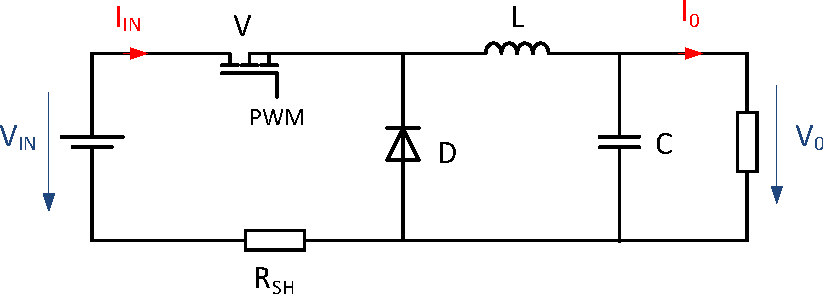
\includegraphics[width=0.90\textwidth]{pics/schema.pdf}
	\caption{Schema Stepdown Converter}
	\label{fig:schema}
\end{figure}

\section{Duty Cycle}
Um den Duty Cycle zu bestimmen sind wir nach folgender Fomel vorgegangen. Im Matlabsktipt haben wir f�r alle Werte, welche in einem gewissen Bereich variieren Matrizen erstellt. Somit k�nnen wir einfach elementweise alle Werte berechnen, ohne mit Loops zu arbeiten. Dies ist viel anschaulicher und besser lesbar. 
\begin{align}
	D =\frac{(V_0 + (R_l + R_0) \cdot I_0 + V_{f0})}{(V_{in} - (R_{DSon} + R_{sh} - R_0) \cdot I_0 + V_{f0})} 
\end{align}

Aus dieser Formel ergibt sich f�r die Ein- bzw. Ausgangsspannung bei 10 Ampere folgende Grafik:

\begin{figure}[ht]
	\centering
		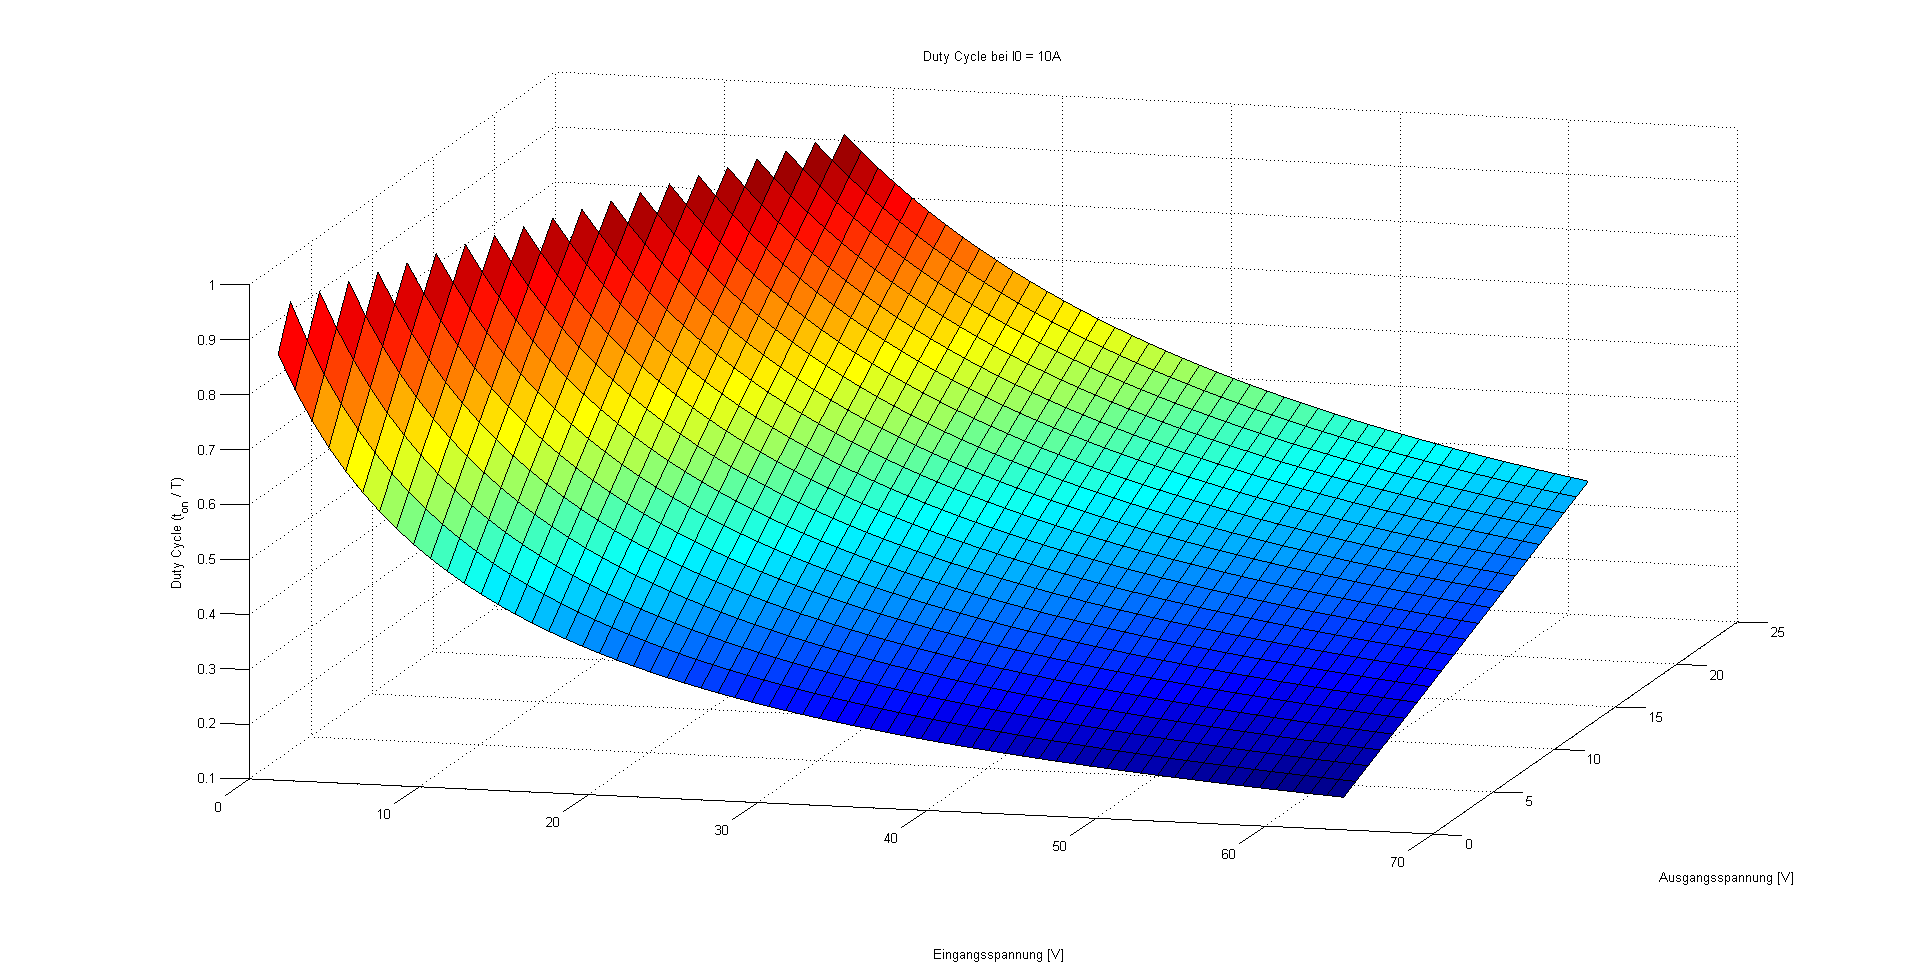
\includegraphics[width=1\textwidth]{pics/DutyCycle.png}
	\caption{Duty Cycle bei 10A}
	\label{fig:Duty Cycle}
\end{figure}
Man erkennt gut, dass dort wo die Ausgangsspannung praktisch gleichgross ist wie die Eingangsspannung der Duty Cycle beinahe eins wird. Dies macht ja auch Sinn, denn in diesem Fall muss der FET immer leiten.

\section{Wirkungsgrad}
Um den Wirkungsgrad zu bestimmen muss zuerst die gesamte Verlustleistung ausgerechnet werden. Dies enth�lt die Schalt-und Leitverluste. Die Leckverluste werden vernachl�ssigt. 
\subsection{Leitverluste}
Die Leitverluste werden mit einfachen Modellen der Bauteile berechnet. Dabei wird z.B. beim MOSFET nur der Drain-Source Widerstand bestimmt und mit dem Quadrat des Effektivwerts des durchfliessenden Stromes multipliziert. 
\subsection{Schaltverluste}


\section{Dimensionierung Drossel}
Die Spule kann berechnet werden, indem man beim maximalen Rippel $\Delta$i (20\% von $I_{0max}$ gew�hlt) die Spannung �ber der Spule bestimmt. 
\begin{align}
	U_L=L\cdot\frac{di}{dt} 
\end{align}
Diese Formel kann f�r kleine $\Delta$i und kurze Zeiten folgendermassen approximiert werden:
\begin{align}
	U_L=L\cdot\frac{\Delta i}{D\cdot T} 
\end{align}
Wobei D der Duty Cycle und T die Periodendauer sind.
Stellt man die Gleichung nach L um und berechnet die Spannung $U_L$ nach Kirchhofschem Maschensatz, eh�lt man die Gleichung:
\begin{align}
	\begin{split}
		L &= \frac{(V_{IN}-V_{0}-(R_{SH}+R_{DSon})\cdot I_0)\cdot D \cdot T}{\Delta i} \\
		&=\frac{(75V-30V-(10m\Omega+2.7m\Omega)\cdot 10A)\cdot 0.4074 \cdot 12.5\mu s}{2A} = 114\mu H
	\end{split}
\end{align}



\subsection{Rippel des Stromes $\Delta$i}

\begin{figure}[ht]
	\centering
		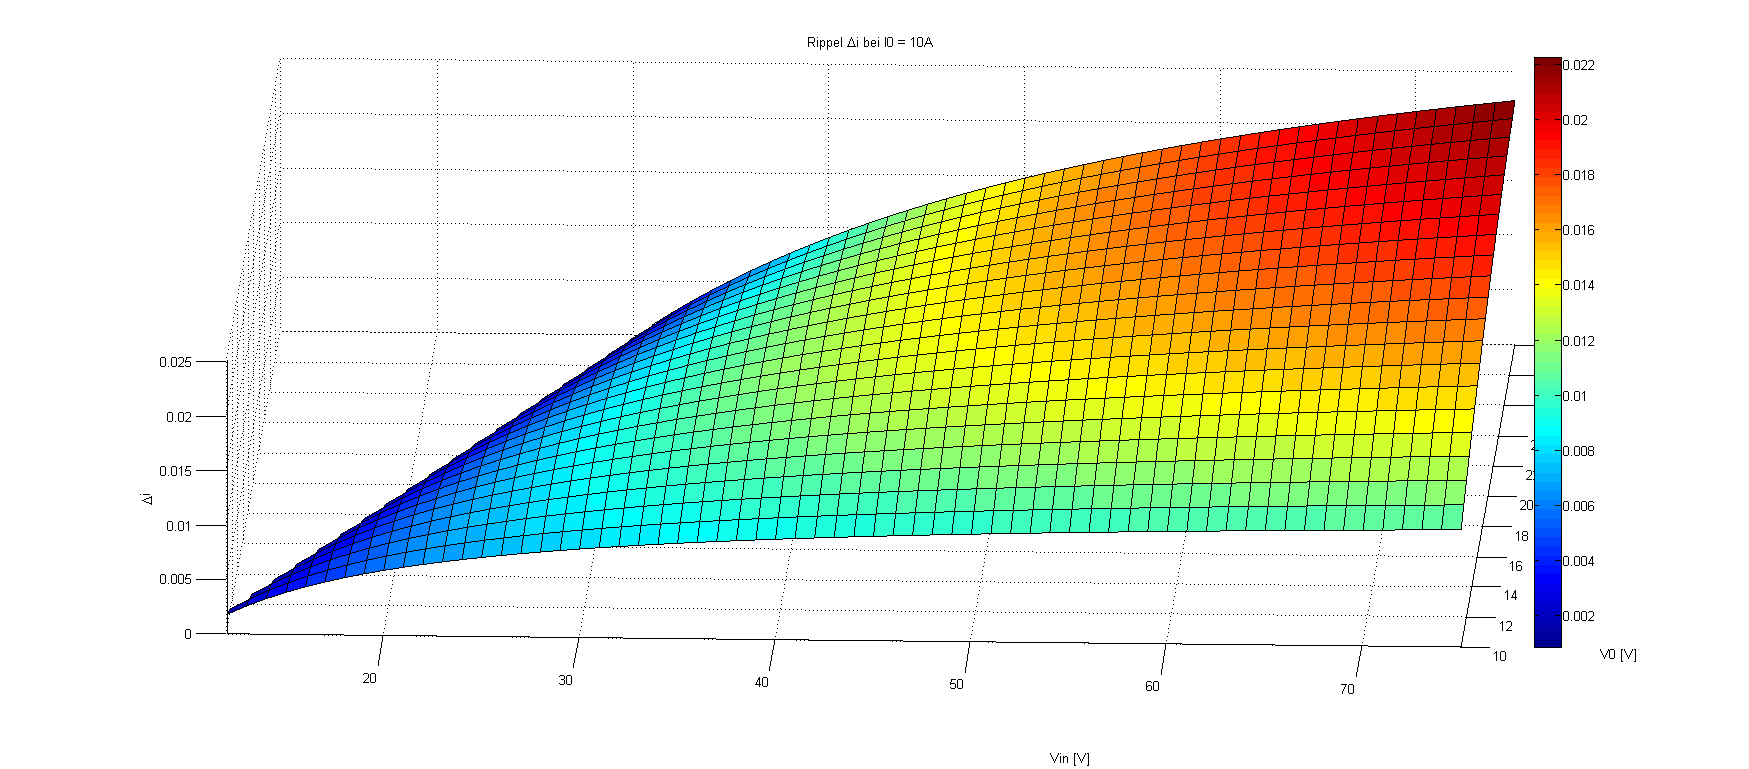
\includegraphics[width=1\textwidth]{pics/Rippel10A.png}
	\caption{Rippel bei 10A}
	\label{fig:Rippel}
\end{figure}

\section{Dimensionierung Kondensator}

%% Der Anhang kommt auf eine neue Zeile
%\newpage
%% Offizielle "A Anhang" Aufz�hlungsvariante
%\appendix
%% Nur im Inhaltsverzeichnis hinzuf�gen (mit richtiger Seite, da vorher "\newpage"), aber kein Text
%\addcontentsline{toc}{section}{Anhang}
%
%% Quellenverzeichnis
%%\addcontentsline{toc}{section}{Quellenverzeichnis}
%\section{Quellenverzeichnis}
%\renewcommand\refname{}
%
%\vspace{-1cm}
%
%\bibliographystyle{amsplain}
%\bibliography{Bildquellen}

\end{document}
